\documentclass[]{elsarticle} %review=doublespace preprint=single 5p=2 column
%%% Begin My package additions %%%%%%%%%%%%%%%%%%%
\usepackage[hyphens]{url}
\usepackage{lineno} % add
\providecommand{\tightlist}{%
  \setlength{\itemsep}{0pt}\setlength{\parskip}{0pt}}

\bibliographystyle{elsarticle-harv}
\biboptions{sort&compress} % For natbib
\usepackage{graphicx}
\usepackage{booktabs} % book-quality tables
%% Redefines the elsarticle footer
%\makeatletter
%\def\ps@pprintTitle{%
% \let\@oddhead\@empty
% \let\@evenhead\@empty
% \def\@oddfoot{\it \hfill\today}%
% \let\@evenfoot\@oddfoot}
%\makeatother

% A modified page layout
\textwidth 6.75in
\oddsidemargin -0.15in
\evensidemargin -0.15in
\textheight 9in
\topmargin -0.5in
%%%%%%%%%%%%%%%% end my additions to header

\usepackage[T1]{fontenc}
\usepackage{lmodern}
\usepackage{amssymb,amsmath}
\usepackage{ifxetex,ifluatex}
\usepackage{fixltx2e} % provides \textsubscript
% use upquote if available, for straight quotes in verbatim environments
\IfFileExists{upquote.sty}{\usepackage{upquote}}{}
\ifnum 0\ifxetex 1\fi\ifluatex 1\fi=0 % if pdftex
  \usepackage[utf8]{inputenc}
\else % if luatex or xelatex
  \usepackage{fontspec}
  \ifxetex
    \usepackage{xltxtra,xunicode}
  \fi
  \defaultfontfeatures{Mapping=tex-text,Scale=MatchLowercase}
  \newcommand{\euro}{€}
\fi
% use microtype if available
\IfFileExists{microtype.sty}{\usepackage{microtype}}{}
\usepackage{graphicx}
% We will generate all images so they have a width \maxwidth. This means
% that they will get their normal width if they fit onto the page, but
% are scaled down if they would overflow the margins.
\makeatletter
\def\maxwidth{\ifdim\Gin@nat@width>\linewidth\linewidth
\else\Gin@nat@width\fi}
\makeatother
\let\Oldincludegraphics\includegraphics
\renewcommand{\includegraphics}[1]{\Oldincludegraphics[width=\maxwidth]{#1}}
\ifxetex
  \usepackage[setpagesize=false, % page size defined by xetex
              unicode=false, % unicode breaks when used with xetex
              xetex]{hyperref}
\else
  \usepackage[unicode=true]{hyperref}
\fi
\hypersetup{breaklinks=true,
            bookmarks=true,
            pdfauthor={},
            pdftitle={Have coaches changed how they select which players to give more minutes to?},
            colorlinks=true,
            urlcolor=blue,
            linkcolor=magenta,
            pdfborder={0 0 0}}
\urlstyle{same}  % don't use monospace font for urls
\setlength{\parindent}{0pt}
\setlength{\parskip}{6pt plus 2pt minus 1pt}
\setlength{\emergencystretch}{3em}  % prevent overfull lines
\setcounter{secnumdepth}{0}
% Pandoc toggle for numbering sections (defaults to be off)
\setcounter{secnumdepth}{0}
% Pandoc header


\usepackage[nomarkers]{endfloat}

\begin{document}
\begin{frontmatter}

  \title{Have coaches changed how they select which players to give more minutes
to?}
    \author[Pontificia Universidad Catolica de Chile]{Derek Corcoran\corref{c1}}
   \ead{derek.corcoran.barrios@gmail.com} 
   \cortext[c1]{Corresponding Author}
    \author[The University of Mississippi]{Nicholas M. Watanabe}
   \ead{nmwatana@olemiss.edu} 
  
      \address[Some Institute of Technology]{Department, Street, City, State, Zip}
    \address[Another University]{Department, Street, City, State, Zip}
  
  \begin{abstract}
  Since the NBA adopted the three point line in 1979 the league has had
  several key rule changes (eg hand checking rules, allowing zone defense)
  that have altered the value of different skill-sets players may have.
  With the creation of the three point shot, a shot made from behind the
  arc was worth more, which made long distance shooting more valuable. We
  explore which stats better explain the minutes per game played in every
  season, to see if coaches have adapted to these rules, all analyses were
  made by possition (Guards, Frowards and Centers). Mostly we see that
  assist per 100 possessions and points per 100 possessions are the two
  stats have the most explanation for minutes per game played. We notice
  that since 2009, rebounding per 100 possessions stopped being an
  important variable selected by coaches
  \end{abstract}
  
 \end{frontmatter}

\emph{Text based on elsarticle sample manuscript, see
\url{http://www.elsevier.com/author-schemas/latex-instructions\#elsarticle}}

\subsection{Methods}\label{methods}

The basketball reference player season finder was used to extract the
per 100 team possessions stats, single season, during the three point
era (since season 1979-80), during the regular season (``Player Season
Finder Basketball-Reference.com'' 2017), and that information was
coupled with the minutes per game played by each player, again extracted
from the basketball reference player season finder but now in the per
game stats. We divided that data-set into 37 data-sets, one for each
season from the 1979-80 season to the 2016-17 season.

\subsection{Queries}\label{queries}

\begin{itemize}
\item
  For single seasons, played in the NBA/BAA, in the regular season, from
  1979-80 to 2016-17, played G or G-F, qualified for Minutes Per Game
  Leaderboard, sorted by descending Win Shares
\item
  For single seasons, played in the NBA/BAA, in the regular season, from
  1979-80 to 2016-17, played F or F-G or F-C, qualified for Minutes Per
  Game Leaderboard, sorted by descending Win Shares
\item
  For single seasons, played in the NBA/BAA, in the regular season, from
  1979-80 to 2016-17, played C or C-F, qualified for Minutes Per Game
  Leaderboard, sorted by descending Win Shares
\end{itemize}

For each season, the per 100 team possession stats was used to fit a
global glm model (Nelder and Baker 1972) that explains the minutes per
game of each player based on the following variables: Two point shot
attempts per 100 possessions, two point shot percentage, three point
shots attempts per 100 possessions, three point shot percentage, free
throw attempts per 100 possessions, free throw percentage, total
rebounds per 100 possessions, assists per 100 possessions, steals per
100 possessions, blocks per 100 possessions, turnovers per 100
possessions, points per 100 possessions and effective field goal
percentage.

In order to be able to compare the strength of relationship of every
variable on the same scale, all of them were scaled and centered (Bro
and Smilde 2003) using the caret package (Kuhn and Johnson 2013).

For each season, we tested variables for collinearity. Then we fitted
every possible first order model not allowing models to coexist if they
had a Pearson correlation coefficient equal or higher than 0.7 (Dormann
et al. 2013). Then the models were ranked based on Akaike's Information
Criteria for small sample sizes (AICc) (Cavanaugh 1997) using the MuMin
Package (Bartoń 2013; Burnham and Anderson 2002). We didn't use model
averaging since even though collinear variables were prohibited to
coexist in the same model, these might coexist in the average model
(Cade 2015), thus we selected the best possible model for each season
selecting by AICc (Burnham and Anderson 2002). All of the analyses using
R statistical Software (Team 2016),

\subsection{Results}\label{results}

\subsubsection{Centers}\label{centers}

As we can see in figure 2, the TRB per hundred possessions is the
variable that appears in most seasons being selected in 38 of 38
seasons, followed by TwoPA per hundred possessions and AST per hundred
possessions being selected in 19 and 12 seasons respectively.

This doesn't hold true for every decade (Figure 1). Specifically, two
point attempts per hundred possessions (TwoPA), where selected in most
seasons (second overall), in the 80s, 90s and 2000s, but in the 2010s,
they go down to the 6th position on times it was selected, with Points
per hundred possessions (pts) takink its place as the second variable
being selected in most seasons only behind Total rebounds per hundred
possessions. Also notably in thee of the last four seasons, Three point
attempts per hundred possessions, was important in determining the
minutes per game a center plays. Even when a variable is selected, that
does not mean is the variable that has the mos strength in a given year,
as an example, if we look at figures 2 and 3, even when Total rebound
per hundred possessions has been selevted for every season in the NBA,
the strength of the relationship of rebounds with minutes per games is
weaker by the year, the same goes for assists. On the other hand, two
point attempts per hundred possessions was selected less times this
decade than any other decade. But when its selected is very strongly
selected.

\begin{figure}[htbp]
\centering
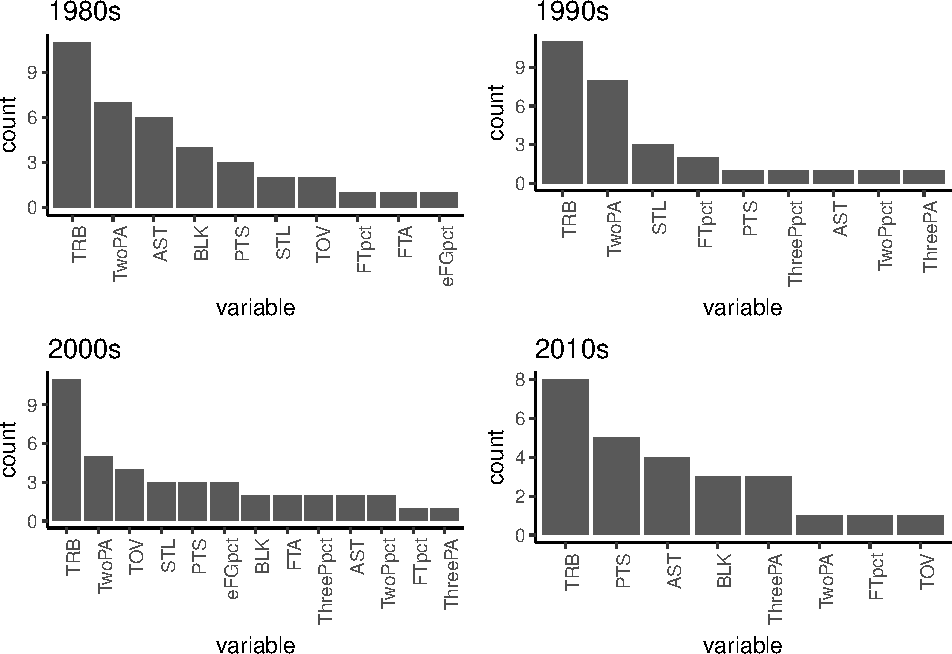
\includegraphics{Coaching_Selection_files/figure-latex/unnamed-chunk-6-1.pdf}
\caption{Times a variable was selected by decade for Centers}
\end{figure}

\begin{figure}[htbp]
\centering
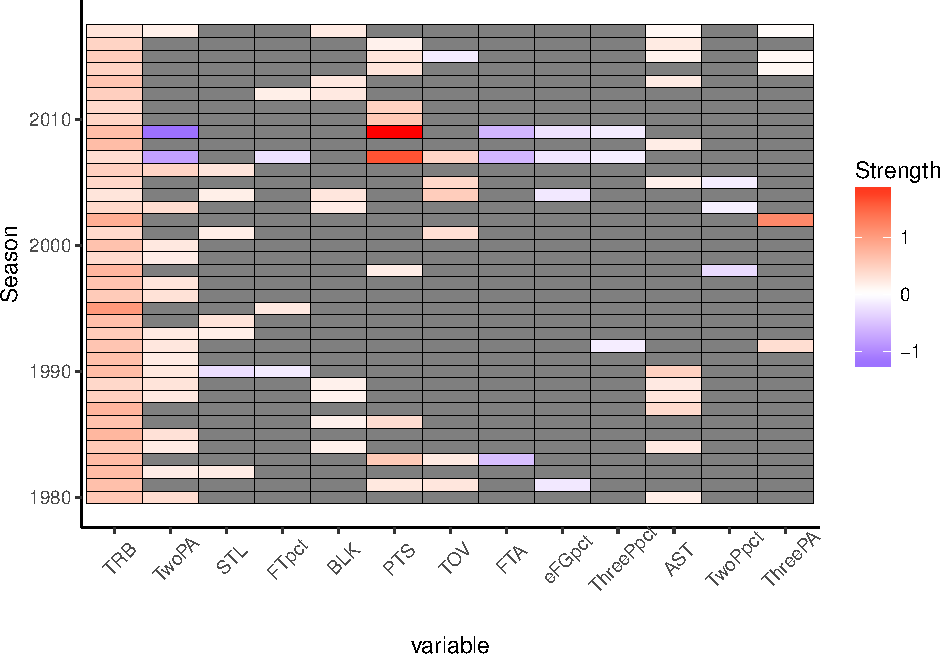
\includegraphics{Coaching_Selection_files/figure-latex/unnamed-chunk-7-1.pdf}
\caption{Strength of relationship by season for Centers}
\end{figure}

\begin{figure}[htbp]
\centering
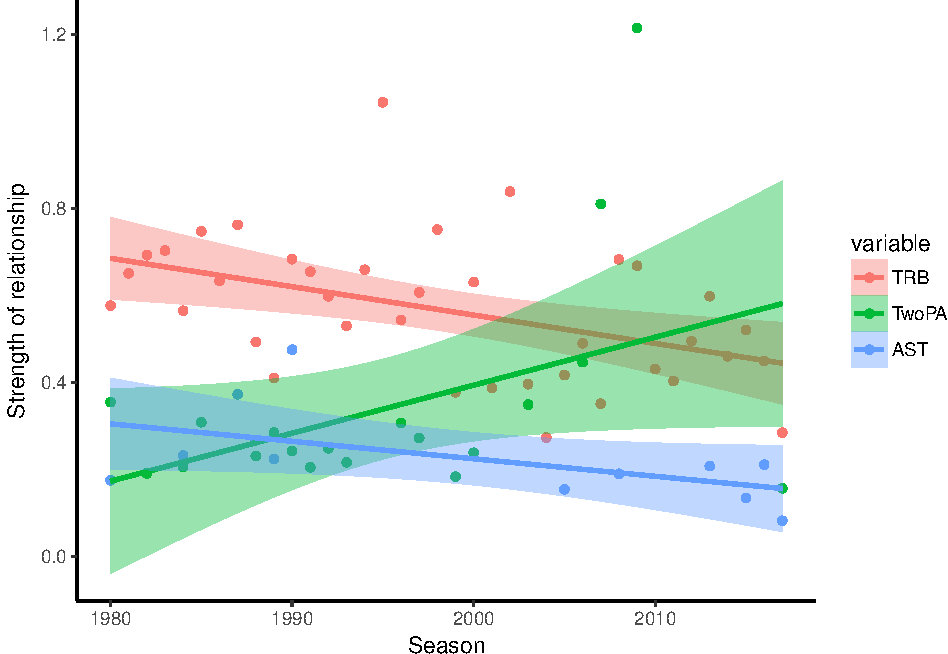
\includegraphics{Coaching_Selection_files/figure-latex/unnamed-chunk-8-1.pdf}
\caption{Strength of relationship by season for assists, Rebounds and
two point attempts per hundred possessions for centers}
\end{figure}

\subsection{Forwards}\label{forwards}

As we can see in figure 5, the TRB per hundred possessions is the
variable that appears in most seasons being selected in 38 of 38
seasons, followed by STL per hundred possessions and TwoPAper hundred
possessions being selected in 28 and 22 seasons respectively.

In this case most notably the change for decades is mostly the Three
point attempts per hundred possessions were chosen in 7 of the last 8
seasons (Figures 4 and 5).

Just as in centers, the total rebounds per hundred possessions have been
less and less important for Frowards to gain minutes per game.

\begin{figure}[htbp]
\centering
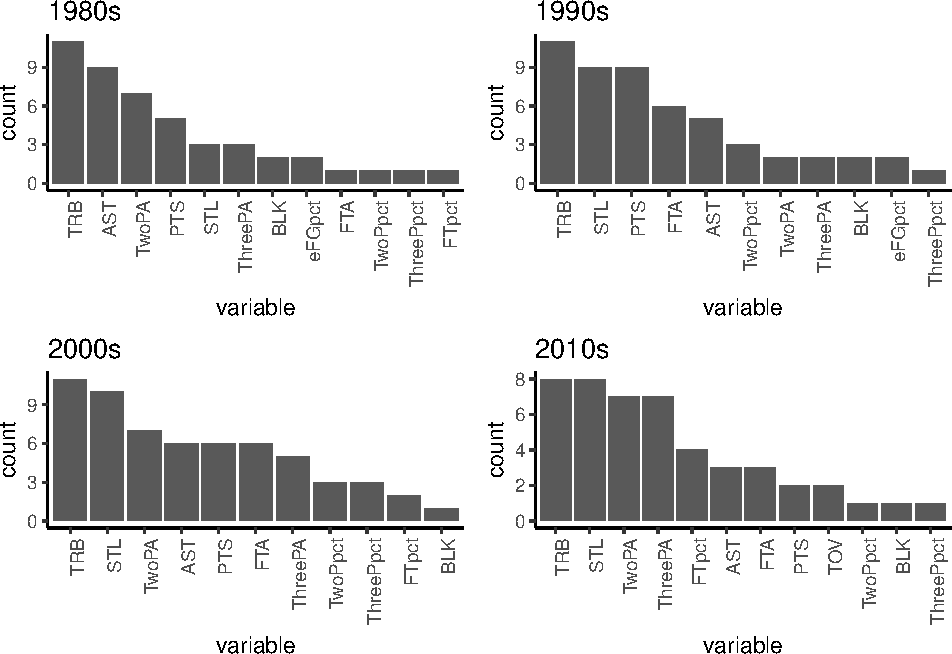
\includegraphics{Coaching_Selection_files/figure-latex/unnamed-chunk-10-1.pdf}
\caption{Times a variable was selected by decade for Forwards}
\end{figure}

\begin{figure}[htbp]
\centering
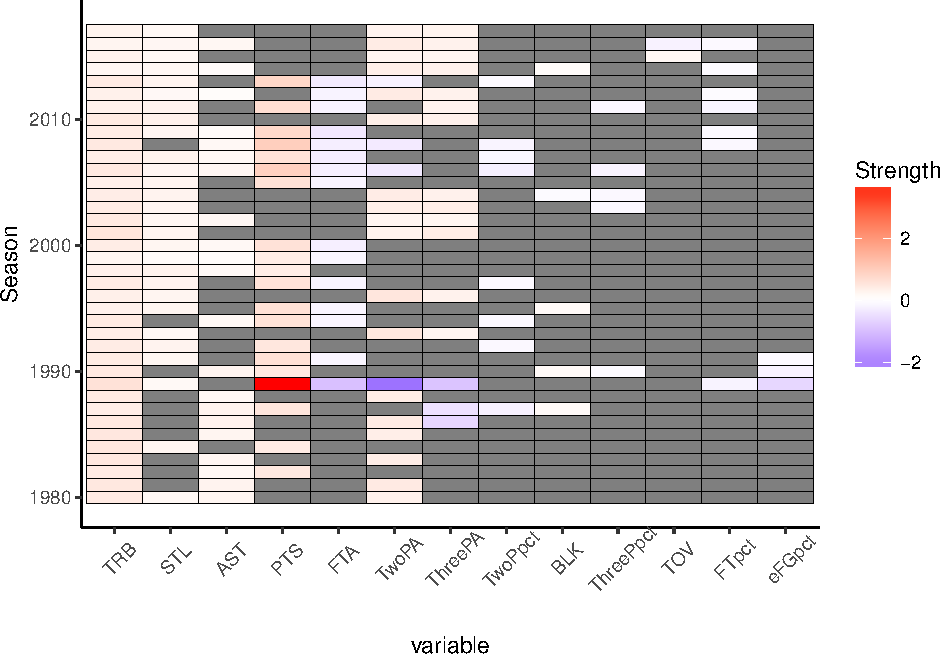
\includegraphics{Coaching_Selection_files/figure-latex/unnamed-chunk-11-1.pdf}
\caption{Strength of relationship by season for Forwards}
\end{figure}

\begin{figure}[htbp]
\centering
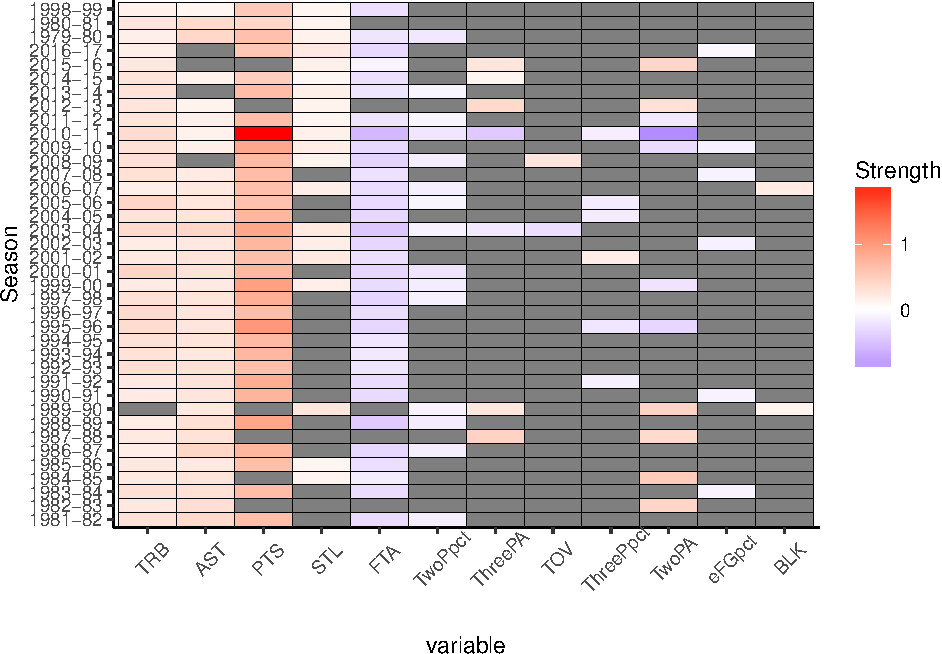
\includegraphics{Coaching_Selection_files/figure-latex/unnamed-chunk-12-1.pdf}
\caption{Strength of relationship by season for assists, Rebounds and
points for Frowards}
\end{figure}

\subsection{Guards}\label{guards}

As we can see in figure 8, the TRB per hundred possessions is the
variable that appears in most seasons being selected in 37 of 38
seasons, followed by AST per hundred possessions and FTA per hundred
possessions being selected in 34 and 33 seasons respectively.

The most striking interdecadal change, is that Assists per hundred
possessions, were the most selected variable through out the 80s and
90s, which falled to 4th most selected in the 2000s and 5th in the 2010s
figure 7. Also, the importance of the variable has greatly decreased

\begin{figure}[htbp]
\centering
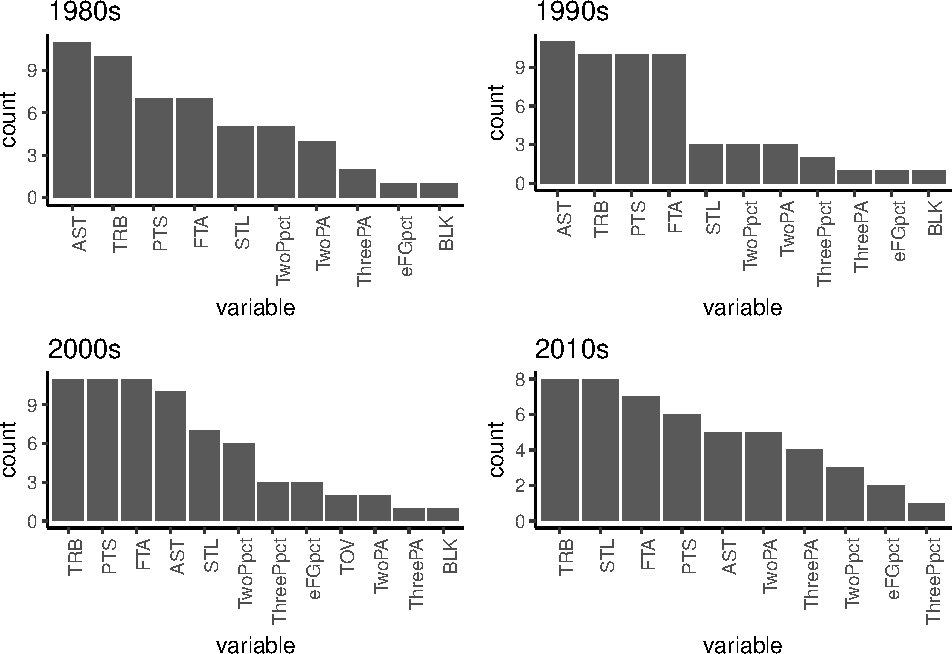
\includegraphics{Coaching_Selection_files/figure-latex/unnamed-chunk-14-1.pdf}
\caption{Times a variable was selected by decade for Guards}
\end{figure}

\begin{figure}[htbp]
\centering
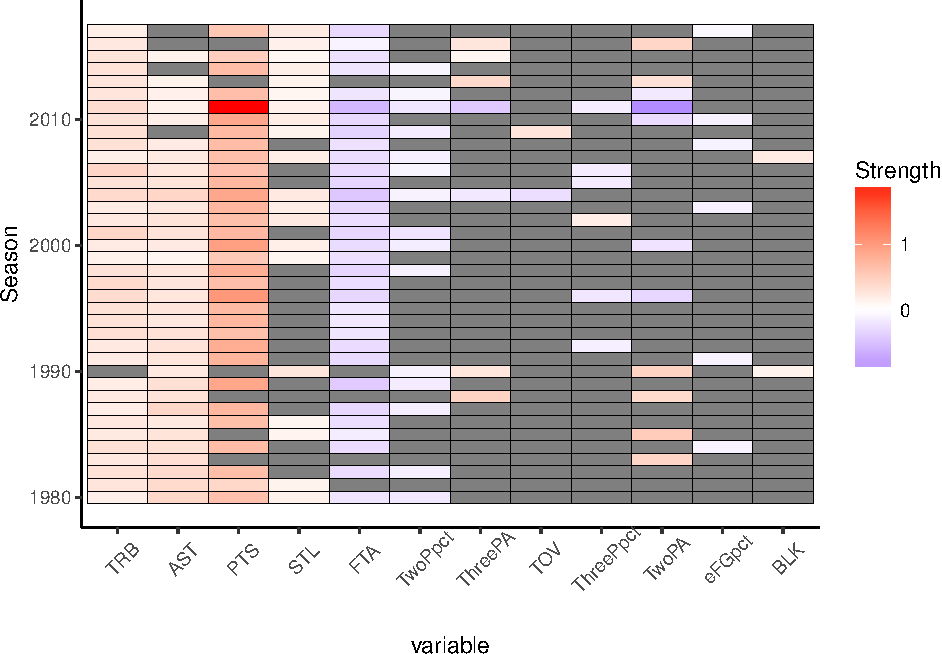
\includegraphics{Coaching_Selection_files/figure-latex/unnamed-chunk-15-1.pdf}
\caption{Strength of relationship by season for Guards}
\end{figure}

\begin{figure}[htbp]
\centering
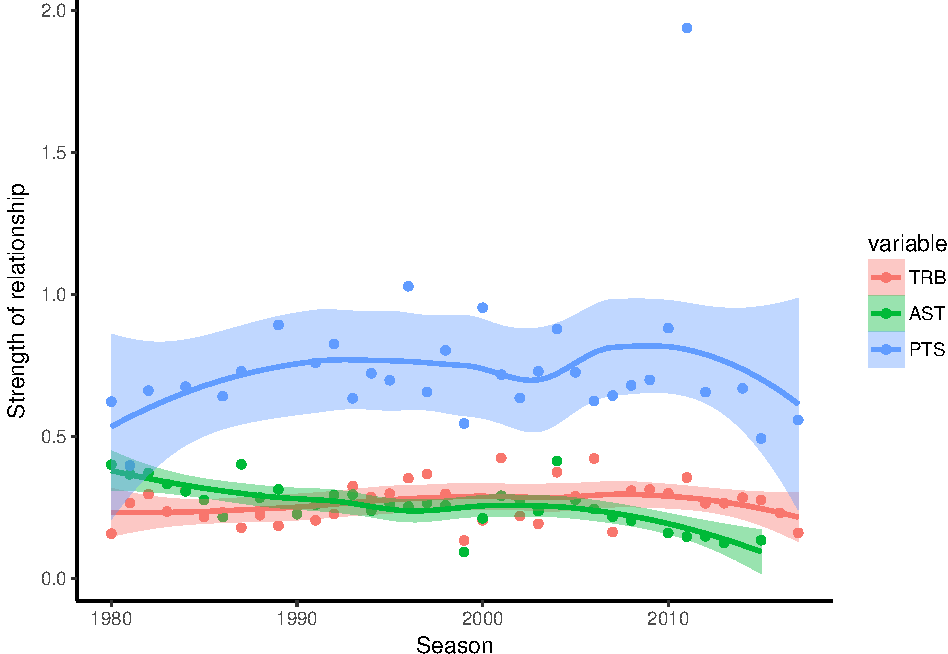
\includegraphics{Coaching_Selection_files/figure-latex/unnamed-chunk-16-1.pdf}
\caption{Strength of relationship by season for assists, Rebounds and
points}
\end{figure}

\paragraph{Functionality}\label{functionality}

The Elsevier article class is based on the standard article class and
supports almost all of the functionality of that class. In addition, it
features commands and options to format the

\begin{itemize}
\item
  document style
\item
  baselineskip
\item
  front matter
\item
  keywords and MSC codes
\item
  theorems, definitions and proofs
\item
  lables of enumerations
\item
  citation style and labeling.
\end{itemize}

\section{Front matter}\label{front-matter}

The author names and affiliations could be formatted in two ways:

\begin{enumerate}
\def\labelenumi{(\arabic{enumi})}
\item
  Group the authors per affiliation.
\item
  Use footnotes to indicate the affiliations.
\end{enumerate}

See the front matter of this document for examples. You are recommended
to conform your choice to the journal you are submitting to.

\section{Bibliography styles}\label{bibliography-styles}

There are various bibliography styles available. You can select the
style of your choice in the preamble of this document. These styles are
Elsevier styles based on standard styles like Harvard and Vancouver.
Please use BibTeX~to generate your bibliography and include DOIs
whenever available.

Here are two sample references: Bartoń (2013; Cade 2015).

\section*{References}\label{references}
\addcontentsline{toc}{section}{References}

\hypertarget{refs}{}
\hypertarget{ref-barton2013mumin}{}
Bartoń, Kamil. 2013. ``MuMIn: Multi-Model Inference. R Package Version
1.9. 13.'' \emph{The Comprehensive R Archive Network (CRAN), Vienna,
Austria}.

\hypertarget{ref-bro2003centering}{}
Bro, Rasmus, and Age K Smilde. 2003. ``Centering and Scaling in
Component Analysis.'' \emph{Journal of Chemometrics} 17 (1). Wiley
Online Library: 16--33.

\hypertarget{ref-burnham2002information}{}
Burnham, KP, and DR Anderson. 2002. ``Information and Likelihood Theory:
A Basis for Model Selection and Inference.'' \emph{Model Selection and
Multimodel Inference: A Practical Information-Theoretic Approach} 2.
Springer-Verlag New York: 49--97.

\hypertarget{ref-cade2015model}{}
Cade, Brian S. 2015. ``Model Averaging and Muddled Multimodel
Inferences.'' \emph{Ecology} 96 (9). Wiley Online Library: 2370--82.

\hypertarget{ref-cavanaugh1997unifying}{}
Cavanaugh, Joseph E. 1997. ``Unifying the Derivations for the Akaike and
Corrected Akaike Information Criteria.'' \emph{Statistics \& Probability
Letters} 33 (2). Elsevier: 201--8.

\hypertarget{ref-dormann2013collinearity}{}
Dormann, Carsten F, Jane Elith, Sven Bacher, Carsten Buchmann, Gudrun
Carl, Gabriel Carré, Jaime R García Marquéz, et al. 2013.
``Collinearity: A Review of Methods to Deal with It and a Simulation
Study Evaluating Their Performance.'' \emph{Ecography} 36 (1). Wiley
Online Library: 27--46.

\hypertarget{ref-kuhn2013applied}{}
Kuhn, Max, and Kjell Johnson. 2013. \emph{Applied Predictive Modeling}.
Vol. 26. Springer.

\hypertarget{ref-nelder1972generalized}{}
Nelder, John A, and R Jacob Baker. 1972. ``Generalized Linear Models.''
\emph{Encyclopedia of Statistical Sciences}. Wiley Online Library.

\hypertarget{ref-BR_2}{}
``Player Season Finder Basketball-Reference.com.'' 2017. Accessed
February 27.
\url{http://www.basketball-reference.com/play-index/psl_finder.cgi}.

\hypertarget{ref-team2016r}{}
Team, R Core. 2016. ``R: A Language and Environment for Statistical
Computing. R Development Core Team, Vienna.''

\end{document}


